\section{Trigger and Data Acquisition System} 
\label{sec:daq}

This section provides a brief summary of the Mu2e Trigger and Data Acquisition (DAQ) subsystem to guide the reader through the rest of this document; more details can be found in Refs.~\cite{Gioiosa:2020tig, Gioiosa:2022dah}. 

\subsection{DAQ system overview}
The DAQ system collects, filters, and monitors the digitized data from the different sub-detectors; delivers the data to online and offline processing for analysis; and synchronizes and controls the detector readout. The DAQ system is based on a “streaming” readout in which all detector data are digitized and zero-suppressed in detector front-end electronics before being transmitted to the DAQ system. While this approach results in a larger data rate, it provides a simpler architecture with greater flexibility in data filtering and monitoring. The DAQ system uses otsdaq~\cite{Biery:2018enl} as a solution, together with the artdaq~\cite{Gioiosa:2020tig} and art~\cite{Green:2012gv} framework to process and filter events. 

An overview of the full system is shown in Figure~\ref{fig:daqoverview}. The major components perform the following functions:
\begin{itemize} 
\item The Readout Controllers (ROC) are reading out, digitizing, and streaming the data from the readout electronics to the DTC. There are 216 ROCs for the tracker, 140 ROCs for the calorimeter, 16 ROCS for the CRV, 1 ROC for the ExtMon, and 1 ROC for the STM. The data, timing signal, and detector control signals are transmitted over a single link from the DTC to tracker/calorimeter ROCs. The timing signal is transported in a separate link for the CRV, while the data are transmitted via ethernet for the monitors. 

\item The Data Transfer Controller (DTC) receives the system clock and event readout request from the CFO and timing fanout module, and reads out data from the ROC. They are installed in the DAQ servers (up to 2 DTCs per server) and are connected to a maximum of 6 ROCs. Each tracker/calorimeter DTC receives the data of a fraction of the detector, and the data are shuffled among the DTCs via Event Building Switches to form a complete event. The data from the CRV are only pulled for requested (triggered) events. 

\item The Command fanout module (CFO) is responsible for generating and synchronizing readout requests. It receives the accelerator zero-crossing marker, supplies a continuous clock to the DTCs, and sends readout request control packets for each system clock. A timing fan-out module is used to broadcast the system clock to drive the transmit link in the chain of DTCs to prevent jitter accumulation

\item The DAQ servers contain the DTCs and run the online trigger software. The DTCs in each server are connected to two different event-building networks. Triggered events are sent to the data logger node, and a dispatcher forwards in a non-blocking way a subset of events to the data quality monitoring nodes. The data from the monitors (STM and ExtMon) are acquired and persisted by separate processes. Slow control monitoring (EPICS) runs on the EPICS host. Communication is performed over two networks: the DCS \& management network and the control \& data storage network. Communication to the lab network is managed by gateway nodes. 
\end{itemize} 

\begin{figure}[htb]
\begin{center}
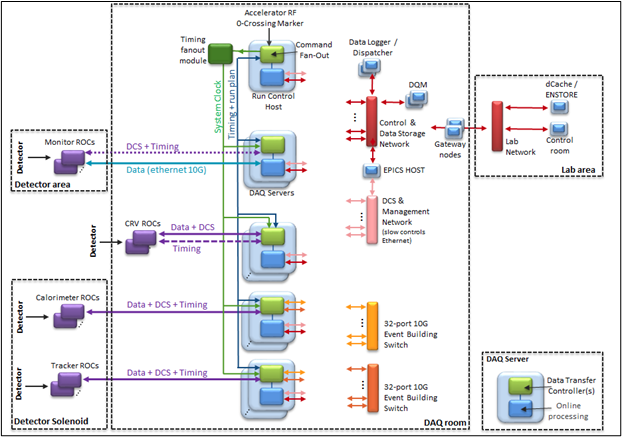
\includegraphics[width=0.9\linewidth]{figures/daq-overview.png}
\caption{Overview of the Mu2e DAQ system}
\label{fig:daqoverview}
\end{center}
\end{figure}

The data flow starts with the tracker and calorimeter DTCs forwarding readout requests from the CFO to their ROCs. The ROCs read out the detector data in response and the DTC collects ROC data for a given Event Window Tag (EWT), a unique tag sent by the CFO to define an event/. Each DTC stores a fraction of the detector data in its memory. The DTCs are grouped into two sets, connected among themselves via an event-building network (in a given server, each DTC is connected to a different network). In each group of DTCs, one DTC acts as an Event Builder for a given EWT, and the remaining DTCs send their data to that DTC via the event-building network. The system is set such that the two halves of an event are built by two DTCs in the same server. The two halves of an event are transferred from the DTCs to the main memory by an ArtdaqBoardReader process, which creates fragments and sends them to the ArtdaqEventBuilder process. The ArtdaqEventBuilder runs the online trigger software on the tracker and calorimeter data. In addition, information from the intensity streams is sent to a data logger. Triggered events are forwarded to a secondary ArtdaqEventBuilder. Information from the CRV is requested via an ArtdaqBoardReader process. The BoardReader instructs the DTC to fetch the corresponding EWT data from the CRV ROCs. A fully assembled event is finally forwarded to a data logger node to be persisted to disk. A dispatcher sends a subset of events in a non-blocking way to the data quality monitoring (DQM) nodes. The dispatcher cannot interrupt data logging; events are simply not forwarded if the DQM nodes are all busy. The DQM metrics are periodically forwarded to the online monitoring nodes. Data acquisition from the monitors follows a similar logic and proceeds independently of the tracker, calorimeter, and CRV. The data are read with their ROCs and forwarded to the corresponding DTCs. Dedicated algorithms are processing and persisting the data to separate files. 
%All data for a given proton pulse are labeled by the same eventID, so that information from the different sources can be correlated in subsequent processing. 

The data will be labeled by a three-part identifier: run, subrun, and event. The DAQ system has been designed to provide deadtimeless transitions between subruns, while transitions between runs incur a deadtime of a few minutes to allow restarting processes and reloading the firmware. The subrun duration is chosen so that conditions are constant throughout the subrun, it spans an integer of MI cycles, and it starts near the end of the $\sim 1$s off-spill period. Subruns will therefore contain both on-spill and off-spill data. The subrun and run duration will be chosen based on operational experience, balancing the size to keep a total number of files manageable while ensuring fast file transfer. At present, the subrun (run) duration is likely to be at the level of a few minutes (6 to 12 hours). For some types of interruptions, a new run might be started when data-taking resumes.

Information about the DAQ/trigger configuration and summary information (e.g. duration of subruns, total number of events processed,...) for each run will be stored in an online run conditions database. Slow-control and other monitoring data are persisted in the EPICS database, and run quality information is similarly recorded. Curated information from online content will be periodically streamed to offline database instances to configure data processing tasks and provide calibration constant required by reconstruction algorithms. This information needs to be available promptly in the offline environment to minimize downstream processing delays. 


\subsection{Data streams}
The data collected by the DAQ will be written in about 15 different file streams (or streams) with information from different sub-systems. These are summarized in Table~\ref{tab:filestreams} and discussed below. A guiding principle is that offline reconstruction avoids reading events from two different streams at the same time. All events from one subrun will be contained within a single physical file to avoid memory bloat when reading sparse skims. However, a single file may contain events from multiple subruns, and two file streams may have different groupings of subruns into files.

\begin{table}[htb]
    \centering
    \begin{tabular}{|l|l|} \hline
Data Type                           & Beam mode \\ \hline
Trk+Cal+CRV triggered events        & On-Spill  \\
Intensity Stream                    & On-Spill  \\
ExtMon data           & On-Spill  \\
Trk+Cal+CRV triggered events        & Off-Spill \\
CRV zero bias triggers              & Off-Spill \\
Calorimeter Pulser Events           & Off-Spill \\ \hline
STM data              & On-Spill + Off-Spill \\ 
Error/Debug Stream                 & On-Spill + Off-Spill \\ \hline
Online DQM output                  & On-Spill + Off-Spill \\
Log files                          & On-Spill + Off-Spill \\ \hline
    \end{tabular}
    \caption{Files streams produced by the Mu2e DAQ.}
\label{tab:filestreams}
\end{table}

The largest stream, triggered on-spill events, contains events selected by the main physics and calibration triggers. The same trigger lines will be run during off-spill periods to record cosmic ray daughters which induce signal-like particles. Additional trigger lines sensitive to through-going cosmic rays passing through the tracker, the calorimeter, or both, will be enabled off-spill. The Intensity stream includes data from proxies to follow fluctuations in the Proton Pulse Intensity for every on-spill event. The Extinction Monitor views a small fraction of the phase space of the scattered proton beam with a pixel telescope and a thick scintillator read out by a PMT (called the Accelerator Fast Feedback). The associated stream produces summary information from these two systems, as well as raw and intermediate data for the pixel tracker. The packaging of summary information remains to be defined but a leading candidate is to collect information for each spill and add a data product summarizing the data in the \art SubRun object. During off-spill data taking, TDAQ plans to record samples of non-zero-suppressed data from a few sectors of the CRV to study pedestals and events in which the calibration signals are injected into the calorimeter and measured. These events will be identified by a bit in the event heartbeat packet and will be written to their own files. The STM will record pulse summary data for every measured pulse and the full waveform for pulses with an energy close to that of the X-ray and gamma-ray lines of interest. Prescaled raw data and pre-processed data will also be written. The STM operates throughout all of the on-spill and off-spill periods in the supercycle. Moreover, the trigger processes will flag events that exhibit unusual behavior and write them into a dedicated Error/Debug stream. For example, selected algorithms might run in a separate thread with a timeout enabled. If the timeout triggers before the algorithm completes, the event will be written to the Debug/Error stream. Finally, the DAQ system will produce online Data Quality Monitoring data and log files, both of which will be saved in their respective streams.


\subsection{Trigger algorithms}
Physics and calibration data are selected by a set of filtering algorithms 
implemented as multiple independent reconstruction paths, each path running one or several reconstruction algorithms. The main physics trigger uses the offline reconstruction algorithms with settings optimizing the timing
performance (see section~\ref{sec:reconstruction}). The artdaq architecture can reuse the output of a given algorithm if it appears in multiple paths, thus minimizing the running time of the online processing. Prescaled factors can be adjusted for each path independently to tune the total trigger rate. Similarly, paths can be enabled or disabled depending on the beam conditions (on-spill or off-spill).   

The main physics trigger is based on information from reconstructed tracks and, to some extent, reconstructed calorimeter clusters. The track reconstruction algorithm is factorized into three main parts:
\begin{itemize}
\item Hits reconstruction from the digitized signals recorded by the tracker. Each signal is transformed into a hit along the tracker wires. A multivariate classifier is used to reject hits produced by a low-momentum Compton electron. 
\item Pattern-recognition to select groups of hits compatible with helicoidal trajectories. Two separate methods are used: a calorimeter-seeded and a tracker-seeded algorithm.
\item Track fit to increase the accuracy of the reconstructed track and improve the background rejection. A simplified Kalman fit is finally performed to improve the accuracy of the reconstructed track parameters and further reject spurious candidates.
\end{itemize}

The resulting efficiency for conversion electrons generating 15 or more hits in the tracker is around 98\% for the nominal proton bunch intensity, with a background rejection factor greater than 1000, and the efficiency only decreases by a few percent for proton bunch intensity up to three times the nominal value. Other trigger streams include for example $\mu^- \rightarrow e^+$ conversion electrons, high-momentum decay-in-orbit electrons, high energy photons produced by radiative pion or muon capture, cosmic rays, or electrons from muons stopping in the internal proton absorber.






